%!TeX spellcheck = en-US
%!TEX root = ../hw2_report.tex
\subsection*{(a) \& (b)}

For all $\alpha$ there is an isolated eigenvalue. All predicted rates of convergence are based on either one circle containing all the eigenvalues or two circles, where one is a point consisting of the outlying eigenvalue. The circles are found in Figure \ref{fig:task2b_1}--\ref{fig:task2b_100}. \\ We observe faster convergence and faster predicted convergence for larger $\alpha$, see Figure  \eqref{fig:task2a_1_5} and Figure \eqref{fig:task2a_10_100}. This is expected, as most eigenvalues are clustered around the origin for $\alpha = 1$. Setting $\alpha = 5$ translates the centre of the cluster away from zero, although some eigenvalues are still close to the origin. Note that we may still have convergence within fewer iterations than the rank of $A$, which is the case for $\alpha = 5$, but not for $\alpha = 1$. For the latter $100$ iterations is required, which is the maximum rank for a $100\times 100$ matrix. As expected the estimated rates of convergence are not of any use and diverges. For $\alpha = 5$ we have convergence and the predicted rates of convergence are indeed bounds, but not very useful due to the underestimation. Furthermore, we see that the predicted rate of convergence for one disc is better than the corresponding for two discs. This is not the case for
$\alpha = 10,\,100$, where we also have faster convergence.





\begin{figure}[h!]
\centering
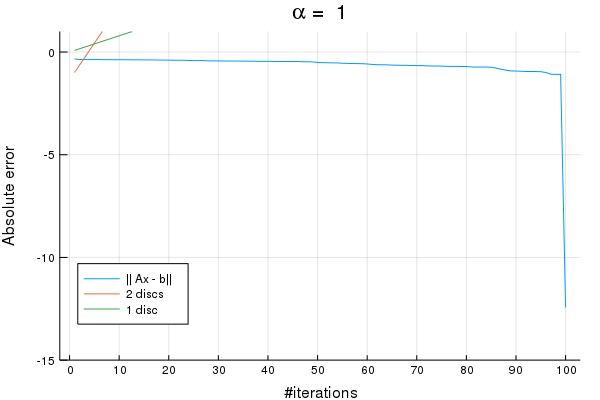
\includegraphics[scale=0.4]{../task2/images/Task2_ab_a1_conv.png}
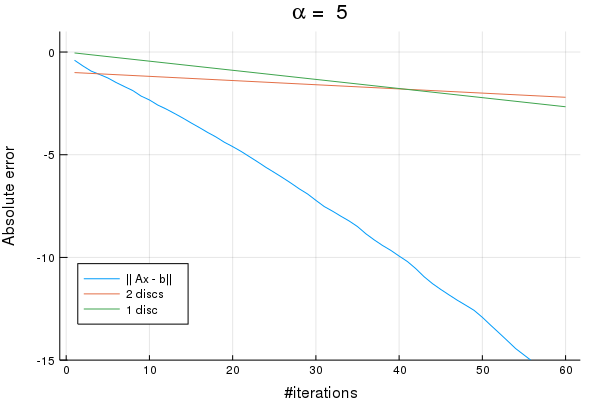
\includegraphics[scale=0.4]{../task2/images/Task2_ab_a5_conv.png}
\caption{Task $1$, (a) \& (b): The convergence of the residual for gmres, plotted against the number of iterations. Here for $\alpha=1$ and $\alpha=5$}
\label{fig:task2a_1_5}
\end{figure}
\begin{figure}[h!]
\centering
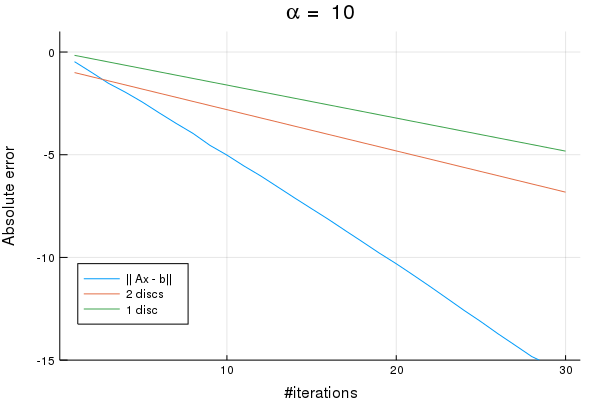
\includegraphics[scale=0.4]{../task2/images/Task2_ab_a10_conv.png}
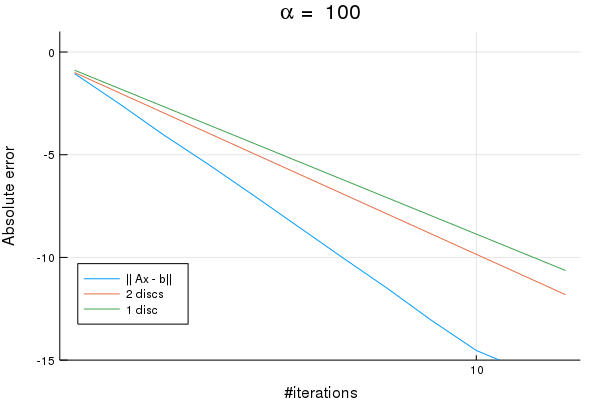
\includegraphics[scale=0.4]{../task2/images/Task2_ab_a100_conv.png}
\caption{Task $1$, (a) \& (b): The convergence of the residual for gmres, plotted against the number of iterations. Here for $\alpha=10$ and $\alpha=100$}
\label{fig:task2a_10_100}
\end{figure}


\begin{figure}[h!]
\centering
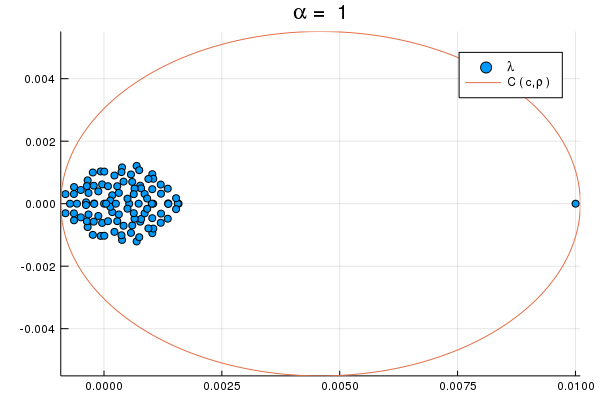
\includegraphics[scale=0.4]{../task2/images/Task2_b_a1_1.png}
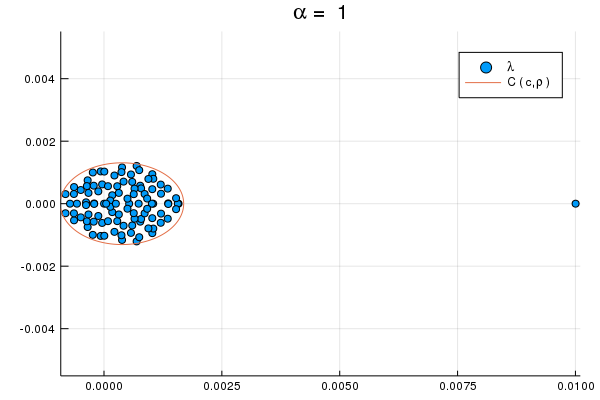
\includegraphics[scale=0.4]{../task2/images/Task2_b_a1_2.png}
\caption{Task $1$, (a) \& (b): For $\alpha = 1$. The two configurations of discs containing all eigenvalues.}
\label{fig:task2b_1}
\end{figure}

\begin{figure}[h!]
\centering
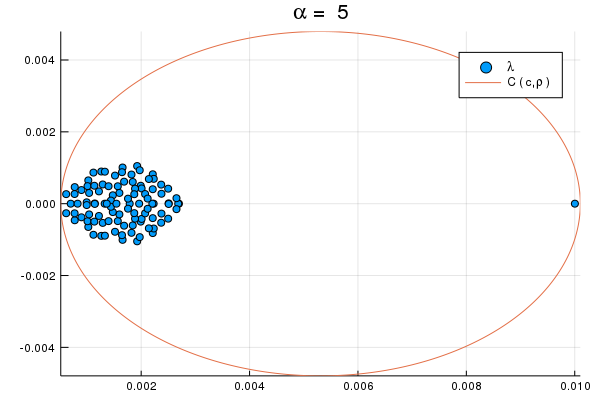
\includegraphics[scale=0.4]{../task2/images/Task2_b_a5_1.png}
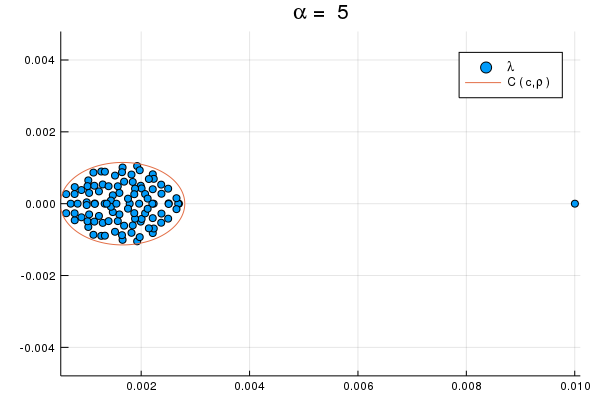
\includegraphics[scale=0.4]{../task2/images/Task2_b_a5_2.png}
\caption{Task $1$, (a) \& (b): For $\alpha = 5$. The two configurations of discs containing all eigenvalues.}
\label{fig:task2b_5}
\end{figure}

\begin{figure}[h!]
\centering
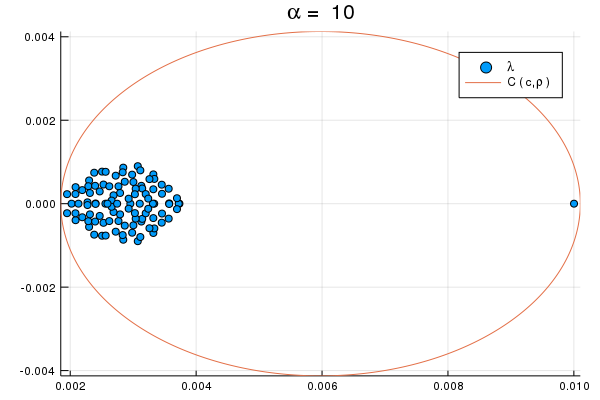
\includegraphics[scale=0.4]{../task2/images/Task2_b_a10_1.png}
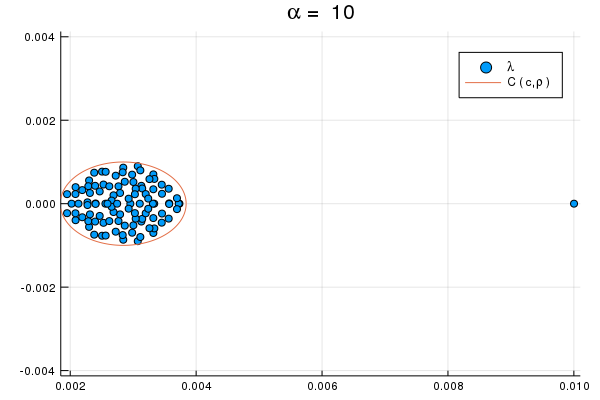
\includegraphics[scale=0.4]{../task2/images/Task2_b_a10_2.png}
\caption{Task $1$, (a) \& (b): For $\alpha = 10$: The two configurations of discs containing all eigenvalues.}
\label{fig:task2b_10}
\end{figure}

\begin{figure}[h!]
\centering
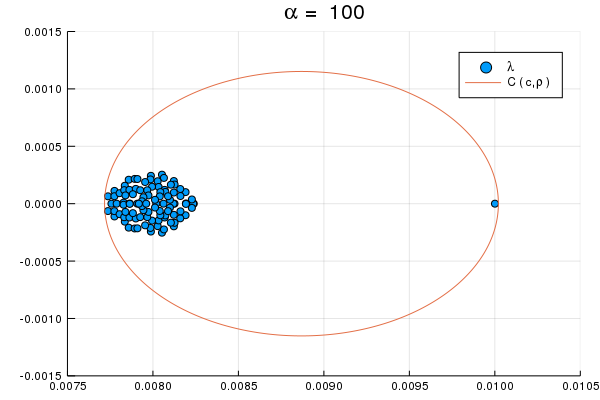
\includegraphics[scale=0.4]{../task2/images/Task2_b_a100_1.png}
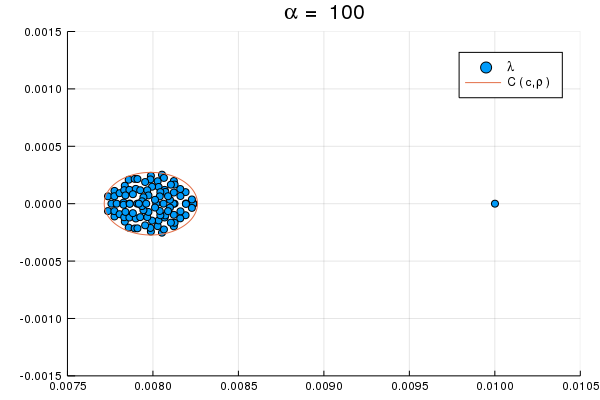
\includegraphics[scale=0.4]{../task2/images/Task2_b_a100_2.png}
\caption{Task $1$, (a) \& (b):  For $\alpha = 100$: The two configurations of discs containing all eigenvalues.}
\label{fig:task2b_100}
\end{figure}
\FloatBarrier
\subsection*{(c)}
See the tables below. For gmres we did $1000$ samples and one evaluation per sample. For backslash the corresponding digits are $3673$ and $1$.

\begin{table}
\centering
\small
\caption{$\alpha = 1$}
\begin{threeparttable}
{\def\arraystretch{1.3}
\begin{tabular}{ccccccccc}
  \toprule
  \multicolumn{9}{c}{\textbf{gmres}}\\
\midrule
& \multicolumn{2}{c}{$m = 100$}&\multicolumn{2}{c}{$m = 200$}&\multicolumn{2}{c}{$m = 500$}&\multicolumn{2}{c}{$m = 1000$}\\
\midrule
& resnorm & time & resnorm & time & resnorm & time &resnorm & time \\
\midrule
n = $5$ & $2.583$ & $162.117$ $\mu $s & $3.848$ & $304.663$ $\mu$s & $6.378$ & $1.511$ ms & $9.0192$ & $3.915$ ms\\
n = $10$ & $2.548$ & $363.392$ $\mu$s & $3.826$ & $591.597$ $\mu$s & $6.326$ & $2.231$ ms & $9.007$ & $8.300$  ms\\
n = 20 & $2.428$ & $1.055$ ms & $3.744$ & $1.439$ ms & $6.307$ & $5.081$ ms & $8.967$ & $16.586$ ms\\
n = 50 & $1.874$ & $5.246$ ms & $3.415$ & $8.117$ ms & $6.194$ & $17.627$ ms & $8.796$ & $48.643$ ms\\
n = 100 & $2.212e-12$ & $28.858$ ms & $2.794$ & $32.087$ ms & $5.718$ & $59.167$ ms & $8.555$ & $133.731$ ms\\
\bottomrule
\multicolumn{9}{c}{\textbf{Backslash}}\\
\midrule
& \multicolumn{2}{c}{$m = 100$} & \multicolumn{2}{c}{$m = 200$} & \multicolumn{2}{c}{$m = 500$} & \multicolumn{2}{c}{$m = 1000$}\\
\midrule
& resnorm & time & resnorm & time & resnorm & time & resnorm & time\\
\midrule
 & $1.056e-12$ & $1.350$ ms & $4.632e-14$ & $6.207$ ms & $1.868e-13$ & $45.407$ ms & $7.074e-13$ & $170.036$ ms \\
\bottomrule

\end{tabular}
}
\end{threeparttable}
\end{table}



\begin{table}
\centering
\small
\caption{$\alpha = 100$}
\begin{threeparttable}
{\def\arraystretch{1.3}
\begin{tabular}{ccccccccc}
  \toprule
  \multicolumn{9}{c}{\textbf{gmres}}\\
\midrule
& \multicolumn{2}{c}{$m = 100$} & \multicolumn{2}{c}{$m = 200$} & \multicolumn{2}{c}{$m = 500$} & \multicolumn{2}{c}{$m = 1000$}\\
\midrule
& resnorm & time & resnorm & time & resnorm & time & resnorm & time \\
\midrule
n = 5 & $6.545e-7$ & $159.159$ $\mu$s & $5.636e-6$ & $291.925$ $\mu$s & $9.712e-5$ & $962.453$ $\mu$s & $6.893e-4$ & $3.790$ ms\\
n = 10 & $1.773e-14$ & $362.841$ $\mu$s & $7.944e-13$ & $564.961$ $\mu$s & $1.667e-10$ & $1.905$ ms & $7.337e-9$ & $7.722$ ms\\
n = 20 & $2.262e-15$ & $1.014$ ms & $4.983e-15$ & $1.712$ ms & $9.328e-15$ & $6.269$ ms & $2.400e-14$ & $16.591$ ms\\
n = 50 & $2.269e-15$ & $5.625$ ms & $5.044e-15$ & $8.152$ ms & $9.291e-15$ & $18.087$ ms & $2.402e-14$ & $58.155$ ms\\
n = 100 & $2.224e-15$ & $30.860$ ms & $5.050e-15$ & $32.769$ ms & $1.030e-14$ & $58.455$ ms & $1.030e-14$ & $61.989$ ms\\
\bottomrule
\multicolumn{9}{c}{\textbf{Backslash}}\\
\midrule
& \multicolumn{2}{c}{$m = 100$} & \multicolumn{2}{c}{$m = 200$} & \multicolumn{2}{c}{$m = 500$} & \multicolumn{2}{c}{$m = 1000$}\\
\midrule
& resnorm & time & resnorm & time &resnorm & time & resnorm & time \\
\midrule
 & $1.662e-15$ & $1.313$ ms & $3.893e-15$ & $5.170$ ms & $7.977e-15$ & $35.644$ ms & $1.565e-14$ & $159.975$ ms\\
\bottomrule

\end{tabular}
}
\end{threeparttable}
\end{table}
\clearpage

\subsection*{(d)}
For $\alpha = 1$ we conclude that the backslash operator is always superior to the gmres method. Based on the results from (b), the convergence is close to none until $n = m$. Then we reach about $1e-14$, thus finding an $n$ such that the relative norm of the residual is about $1e-5$ is not feasible.\\

For $\alpha = 100$ the situation is different. To obtain the relative residual norm the errors in the table should be scaled by $6$, $8$, $13$ and $18$. Then all errors, except for the one corresponding to $m = 1000$ is below $1e-5$. However, setting $n = 6$ gives a relative residual norm of $1e-6$ for $m = 1000$ as well. Moreover, gmres is faster: for $n = 5$ the realtive timings $t_{\text{gmres}}/t_{\text{backslash}}$ are: $0.159$,  $0.0582$,  $0.0274857$ and  $0.0238365$.
